
%(BEGIN_QUESTION)
% Copyright 2011, Tony R. Kuphaldt, released under the Creative Commons Attribution License (v 1.0)
% This means you may do almost anything with this work of mine, so long as you give me proper credit

One of the major processes used to treat municipal wastewater is {\it aeration}, where the dissolved oxygen concentration of the wastewater is increased by bubbling air through the water in an {\it aeration basin}.  A dissolved oxygen (``DO'') analyzer measures the oxygen concentration in the wastewater, and a controller varies the speeds of blowers pumping air into the basins using AC motors powered through variable-frequency drives (VFDs) which allow the controllers' 4-20 mA output signals command the motors how fast to spin:

$$\includegraphics[width=15.5cm]{i00776x01.eps}$$

Identify the proper actions for each controller in this system, assuming direct-acting transmitters and VFDs that spin the motor at a faster speed with a greater 4-20 mA signal:

\vskip 10pt

AIC-25 = {\it direct} or {\it reverse}? \hskip 30pt FIC-18 = {\it direct} or {\it reverse}? \hskip 30pt FIC-19 = {\it direct} or {\it reverse}?

\vskip 10pt

Suppose an operator calls you to examine this system and determine why the dissolved oxygen value is not holding at setpoint.  According to the operator, everything was working fine yesterday, and had been working fine for months.  You go to the control room to view the display on the DCS, and you find these values:

% No blank lines allowed between lines of an \halign structure!
% I use comments (%) instead, so that TeX doesn't choke.

$$\vbox{\offinterlineskip
\halign{\strut
\vrule \quad\hfil # \ \hfil & 
\vrule \quad\hfil # \ \hfil & 
\vrule \quad\hfil # \ \hfil & 
\vrule \quad\hfil # \ \hfil \vrule \cr
\noalign{\hrule}
%
% First row
{\bf Parameter} & {\bf AIC-25} & {\bf FIC-18} & {\bf FIC-19} \cr
%
\noalign{\hrule}
%
% Another row
PV & 41\% & 99\% & 2\% \cr
%
\noalign{\hrule}
%
% Another row
SP & 75\% & 100\% & 100\% \cr
%
\noalign{\hrule}
%
% Another row
Output & 100\% & 82\% & 100\% \cr
%
\noalign{\hrule}
} % End of \halign 
}$$ % End of \vbox

Identify {\it two} different faults, each one independently capable of accounting for all symptoms evident in this table.

\begin{itemize}
\item{} 
\vskip 50pt
\item{} 
\end{itemize}

\underbar{file i00776}
%(END_QUESTION)




%(BEGIN_ANSWER)

{\it Two points for AIC action, 1 point each for FIC actions.  3 points each for valid faults.}

\vskip 10pt

AIC-25 = {\bf reverse} \hskip 50pt FIC-18 = {\bf reverse} \hskip 50pt FIC-19 = {\bf reverse}

\vskip 10pt

The problem lies within the FIC-19 blower/nozzle system.  Possibilities include:

\begin{itemize}
\item{} Plugged nozzle array
\item{} Plugged silencer
\item{} VFD power tripped (off)
\item{} Blower failed (not blowing air)
\end{itemize}

%(END_ANSWER)





%(BEGIN_NOTES)

{\bf This question is intended for exams only and not worksheets!}.

%(END_NOTES)


